\documentclass{article}

\usepackage{amsmath,amssymb}
\usepackage{tikz}
\usepackage{pgfplots}
\usepackage{xcolor}
\usepackage[left=2.1cm,right=3.1cm,bottom=3cm,footskip=0.75cm,headsep=0.5cm]{geometry}
\usepackage{enumerate}
\usepackage{enumitem}
\usepackage{marvosym}
\usepackage{tabularx}
\usepackage{parskip}

\usepackage{listings}
\definecolor{lightlightgray}{rgb}{0.95,0.95,0.95}
\definecolor{lila}{rgb}{0.8,0,0.8}
\definecolor{mygray}{rgb}{0.5,0.5,0.5}
\definecolor{mygreen}{rgb}{0,0.8,0.26}
\lstdefinestyle{java} {language=java}
\lstset{language=java,
	basicstyle=\ttfamily,
	keywordstyle=\color{lila},
	commentstyle=\color{lightgray},
	stringstyle=\color{mygreen}\ttfamily,
	backgroundcolor=\color{white},
	showstringspaces=false,
	numbers=left,
	numbersep=10pt,
	numberstyle=\color{mygray}\ttfamily,
	identifierstyle=\color{blue},
	xleftmargin=.1\textwidth, 
	%xrightmargin=.1\textwidth,
	escapechar=§,
	%literate={\t}{{\ }}1
}

\usepackage[utf8]{inputenc}

\renewcommand*{\arraystretch}{1.4}

\newcolumntype{L}[1]{>{\raggedright\arraybackslash}p{#1}}
\newcolumntype{R}[1]{>{\raggedleft\arraybackslash}p{#1}}
\newcolumntype{C}[1]{>{\centering\let\newline\\\arraybackslash\hspace{0pt}}m{#1}}

\newcommand{\E}{\mathbb{E}}
\DeclareMathOperator{\rk}{rk}
\DeclareMathOperator{\Var}{Var}
\DeclareMathOperator{\Cov}{Cov}

\title{\textbf{INLOOP Softwaretechnologie, Linked List}}
\author{\textsc{Henry Haustein}}
\date{}

\begin{document}
	\maketitle
	
	\section*{vollständiger Code}
	Datei \texttt{ListElement.java}
	\begin{lstlisting}[style=java,tabsize=2]
public class ListElement {
	private String content;
	private ListElement next;
	
	public ListElement(String con) {
		if(con == null || con.equals("")) {
			throw new IllegalArgumentException("content must not be null");
		}
		else {
			this.content = con;
			this.next = null;
		}
	}
	
	public String getContent() {
		return content;
	}
	
	public ListElement getNext() {
		return next;
	}
	
	public void setContent(String con) {
		if(con == null || con.equals("")) {
			throw new IllegalArgumentException("content must not be null");
		}
		else {
			content = con;
		}
	}
	
	public void setNext(ListElement nx) {
		next = nx;
	}
}
	\end{lstlisting}

	Datei \texttt{List.java}
	\begin{lstlisting}[style=java,tabsize=2]
public class List {
	private ListElement head;
	
	public List() {
		this.head = null;
	}
	
	public void append(String con) {
		ListElement elem = new ListElement(con);
		
		// 0 Elements
		if(head == null) {
			head = elem;
		}
		else {
			// 1 Element = head
			if(head.getNext() == null) {
				head.setNext(elem);
			}
			// more than 1 Element
			else {
				ListElement current = head;
				while(current != null) {
					if(current.getNext() == null) {
						System.out.println("Found end at " + current.getContent());
						current.setNext(elem);
						break;
					}
					else {
						System.out.println("Go to next element of " + current.getContent());
						current = current.getNext();
					}
					
				}
			}
		}
	}
	
	public String remove(String toRemove) {
		if(toRemove == null || toRemove.equals("")) {
			throw new IllegalArgumentException("content must not be null");
		}
		
		// 0 Elements
		if(head == null) {
			return null;
		}
		else {
			// 1 Element
			if(head.getNext() == null) {
				if(head.getContent().equals(toRemove)) {
					String content = head.getContent();
					head = null;
					return content;
				}
				else {
					return null;
				}
			}
			// more than 1 Element
			else {
				// must head be removed ?
				if(head.getContent().equals(toRemove)) {
					String content = head.getContent();
					head = head.getNext();
					return content;
				}
				else {
					ListElement current = head.getNext();
					ListElement prev = head;
					while(true) {
						if(current.getContent().equals(toRemove)) {
							prev.setNext(current.getNext());
							return current.getContent();
						}
						else {
							if(current.getNext() == null) {
								return null;
							}
							else {
								prev = current;
								current = current.getNext();
							}
						}
					}
				}
			}
		}
	}
	
	public void printList() {
		if(head == null) {
			System.out.println("List is empty");
		}
		else {
			ListElement current = head;
			while(current != null) {
				System.out.println(current.getContent());
				current = current.getNext();
			}
		}
	}
	
}
	\end{lstlisting}

	\section*{Erklärung}
	Auch hier ist die Klasse \texttt{ListElement} recht klar, der Operator \texttt{||} steht für "oder"\footnote{Der Operator \texttt{\&\&} steht für "and".}.
	
	Die Idee hinter der \texttt{append()}-Funktion ist, dass es für das Anfügen an eine Liste eigentlich nur 2 Fälle gibt:
	\begin{itemize}
		\item Die Liste ist leer, dass besteht die neue Liste nur aus dem angefügten Objekt.
		\item Die Liste ist nicht leer, wir müssen also das letzte Element finden, und hängen an dieses Element das anzufügende Element dran.
	\end{itemize}
	Ich habe hier tatsächlich noch mal eine Unterscheidung gemacht, ob die Liste nur aus einem Element besteht, oder ob es noch mehr Elemente gibt. Eigentlich sollte diese Unterscheidung nicht notwendig sein und ich denke auch, dass mein Code ohne Probleme funktionieren sollte, wenn man die Zeilen 16 bis 21 aus meinem Quelltext entfernt, aber der Code funktioniert. Wissen wir nun, dass die Liste mehr als ein Element enthält, so setzen wir unser aktuell betrachtetes Element auf \texttt{head}. Wir gehen nun solange zum Nachfolger des aktuell betrachteten Elements, bis wir feststellen, dass das aktuelle Element keinen Nachfolger hat, also \texttt{current.getNext() == null}. Das verhindert auch, dass die Bedingung in der while-Schleife jemals falsch sein wird, ich hätte auch also auch \texttt{while(true)} statt \texttt{while(current != null)} schreiben können. Haben wir nun das letzte Element gefunden, so können wir an dieses den Nachfolger dranhängen und brechen die while-Schleife ab.
	
	Die \texttt{remove()}-Funktion ist noch komplizierter. Grundsätzliche Idee ist auch hier, dass wir überprüfen, ob der Nachfolger des aktuell betrachteten Elements gelöscht werden muss. Wenn dem so ist, müssen wir den Nachfolger des aktuell betrachteten Elements auf \texttt{null} setzen. Das impliziert, dass diese Vorgehensweise nur dann funktioniert, wenn in der Liste mindestens 2 Elemente sind, wir müssen also die Fälle mit 0 Elementen in der Liste und mit einem Element in der Liste separat bearbeiten.
	\begin{itemize}
		\item Wenn es keine Elemente in der Liste gibt, so kann auch nichts entfernt werden, und wir geben \texttt{null} zurück.
		\item Ist nur ein Element in der Liste, so müssen wir überprüfen, ob dieses gelöscht werden muss. Ist dem so, so muss die ganze Liste gelöscht werden (\texttt{head = null;}). Vorher haben ich noch den Inhalt von \texttt{head} abgespeichert, so dass ich ihn nach dem Löschen der Liste zurückgeben kann.
	\end{itemize}
	Ein weiterer Spezialfall ist, dass die Liste mehr als 1 Element enthält, aber das erste Element gelöscht werden muss. In diesem Fall muss man die \texttt{head}-Variable einfach auf das zweite Listenelement setzen. Sind nun diese ganzen Spezialfälle nicht eingetreten, so setzen wir die Variable \texttt{current} auf das zweite Element der Liste und die Variable \texttt{prev} (wie \textit{previous}, also Vorgänger) auf das erste Element der Liste. Die Variablenbezeichnung mag vielleicht etwas unintuitiv sein, aber das Element, was in \texttt{current} drin steht, soll auf Löschbarkeit überprüft werden, und in dem Fall, dass dieses gelöscht werden muss, darf der Vorgänger dieses Elements nicht mehr auf \texttt{current} zeigen, sondern muss auf \texttt{current.getNext()} zeigen.
	\begin{center}
		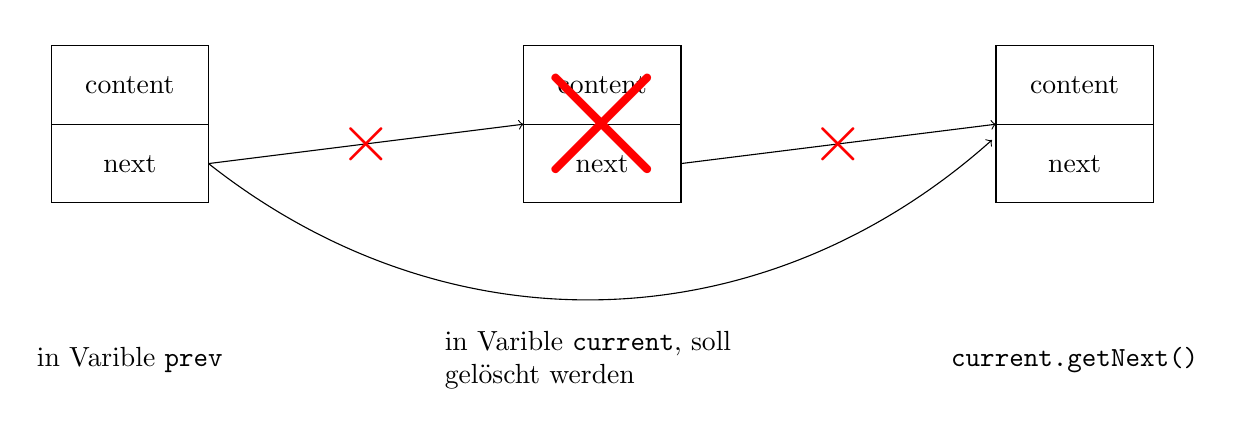
\begin{tikzpicture}
			\draw (0,0) rectangle (2,-1) node[pos=0.5] {content};
			\draw (0,-1) rectangle (2,-2) node[pos=0.5] {next};
			
			\draw (6,0) rectangle (8,-1) node[pos=0.5] {content};
			\draw (6,-1) rectangle (8,-2) node[pos=0.5] {next};
			
			\draw (12,0) rectangle (14,-1) node[pos=0.5] {content};
			\draw (12,-1) rectangle (14,-2) node[pos=0.5] {next};
			
			\draw[->] (2,-1.5) -- (6,-1);
			\draw[->] (2,-1.5) to[bend right=40] (11.95,-1.2);
			\draw[->] (8,-1.5) -- (12,-1);
			
			\node[red,scale=3] at (7,-1) {\Huge$\times$};
			\node[red] at (4,-1.25) {\Huge$\times$};
			\node[red] at (10,-1.25) {\Huge$\times$};
			
			\node at (1,-4) {in Varible \texttt{prev}};
			\node[text width=4cm] at (7,-4) {in Varible \texttt{current}, soll gelöscht werden};
			\node at (13,-4) {\texttt{current.getNext()}};
		\end{tikzpicture}
	\end{center}
	Sind wir am Ende der Liste angekommen (\texttt{current.getNext() == null}), ohne etwas zu finden, so geben wir \texttt{null} zurück. Gibt es hingegen noch einen Nachfolger, so updaten wir \texttt{prev} und \texttt{current}.
	
	Zu Testzwecken habe ich mir noch eine Funktion \texttt{printList()} geschrieben, die sich durch die Liste iteriert und einfach den Inhalt der einzelnen Elemente ausgibt.
	
	
\end{document}